\documentclass[border=5pt]{standalone}
\usepackage{pgfplots}
\pgfplotsset{compat=1.18}
\usepackage{siunitx}
\usepackage{tikz}
\usetikzlibrary{calc}

\definecolor{barblue}{RGB}{31,119,180}
\definecolor{barorange}{RGB}{255,127,14}

\begin{document}

% Chart 1: Total Training Time
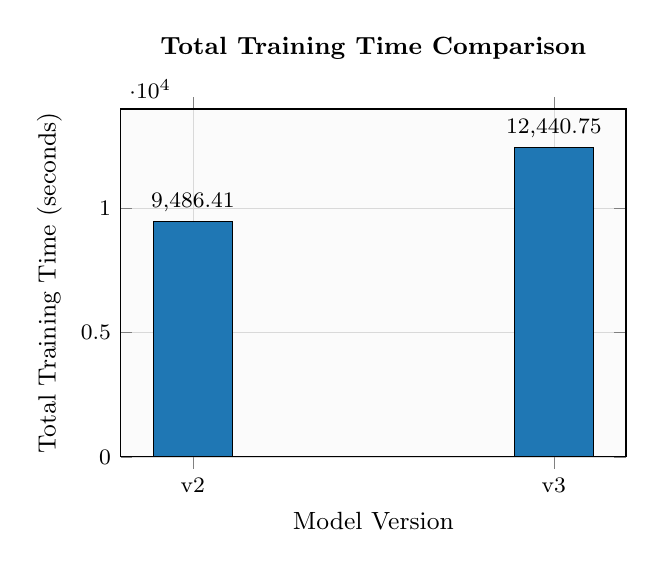
\begin{tikzpicture}
    \begin{axis}[
        width=8cm,
        height=6cm,
        ybar,
        bar width=1cm,
        xlabel={Model Version},
        ylabel={Total Training Time (seconds)},
        symbolic x coords={v2,v3},
        xtick=data,
        ymin=0,
        ymax=14000,
        nodes near coords,
        nodes near coords align={vertical},
        every node near coord/.style={font=\footnotesize},
        grid=both,
        grid style={line width=.1pt, draw=gray!10},
        major grid style={line width=.2pt,draw=gray!30},
        title={Total Training Time Comparison},
        axis background/.style={fill=gray!3},
        title style={yshift=3mm, font=\small\bfseries},
        label style={font=\small},
        tick label style={font=\footnotesize},
        enlarge x limits=0.2
    ]
    \addplot[fill=barblue] coordinates {
        (v2, 9486.41)
        (v3, 12440.75)
    };
    \end{axis}
\end{tikzpicture}

\hspace{0.5cm}

% Chart 2: Number of Parameters
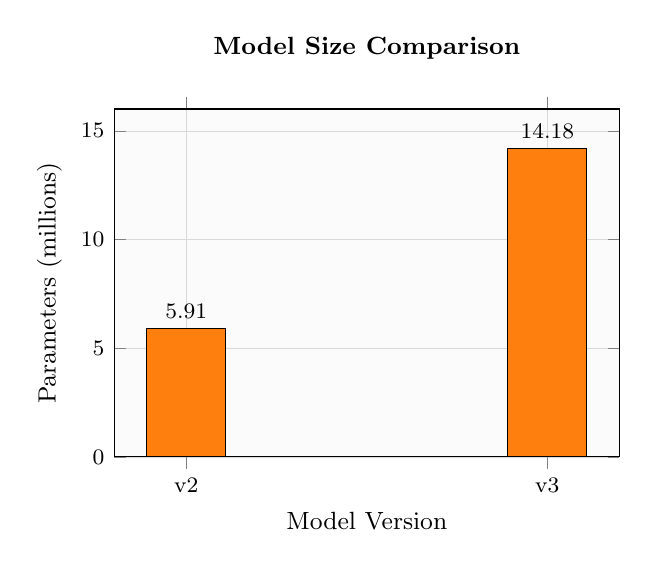
\begin{tikzpicture}
    \begin{axis}[
        width=8cm,
        height=6cm,
        ybar,
        bar width=1cm,
        xlabel={Model Version},
        ylabel={Parameters (millions)},
        symbolic x coords={v2,v3},
        xtick=data,
        ymin=0,
        ymax=16,
        nodes near coords,
        nodes near coords align={vertical},
        every node near coord/.style={font=\footnotesize},
        grid=both,
        grid style={line width=.1pt, draw=gray!10},
        major grid style={line width=.2pt,draw=gray!30},
        title={Model Size Comparison},
        axis background/.style={fill=gray!3},
        title style={yshift=3mm, font=\small\bfseries},
        label style={font=\small},
        tick label style={font=\footnotesize},
        enlarge x limits=0.2
    ]
    \addplot[fill=barorange] coordinates {
        (v2, 5.91)
        (v3, 14.18)
    };
    \end{axis}
\end{tikzpicture}

\hspace{0.5cm}

% Chart 3: Final CER
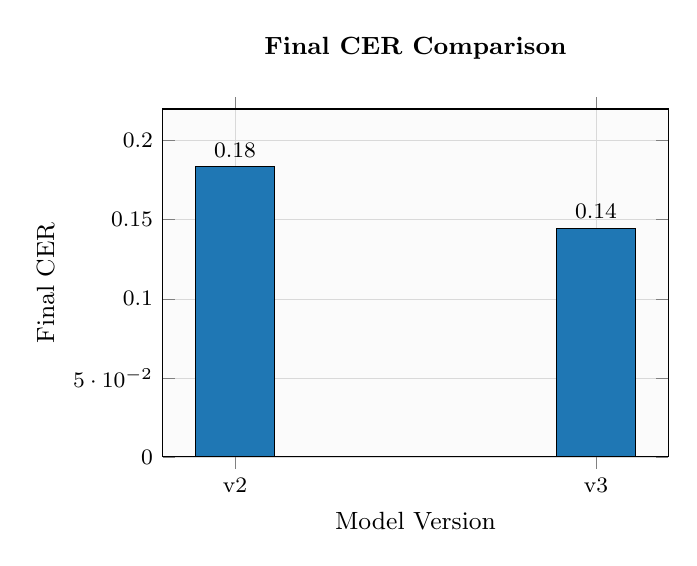
\begin{tikzpicture}
    \begin{axis}[
        width=8cm,
        height=6cm,
        ybar,
        bar width=1cm,
        xlabel={Model Version},
        ylabel={Final CER},
        symbolic x coords={v2,v3},
        xtick=data,
        ymin=0,
        ymax=0.22,
        nodes near coords,
        nodes near coords align={vertical},
        every node near coord/.style={font=\footnotesize},
        grid=both,
        grid style={line width=.1pt, draw=gray!10},
        major grid style={line width=.2pt,draw=gray!30},
        title={Final CER Comparison},
        axis background/.style={fill=gray!3},
        title style={yshift=3mm, font=\small\bfseries},
        label style={font=\small},
        tick label style={font=\footnotesize},
        enlarge x limits=0.2
    ]
    \addplot[fill=barblue] coordinates {
        (v2, 0.1834)
        (v3, 0.1447)
    };
    \end{axis}
\end{tikzpicture}

\end{document}
